\documentclass[12pt]{book}
% Page geometry
\usepackage[acronym, toc]{glossaries}
\usepackage[a4paper,top=3cm,bottom=3cm,left=3.25cm,right=3.25cm]{geometry}

% Fonts and Language
\usepackage[T1]{fontenc}
\usepackage{libertine}
\usepackage[english]{babel}
\usepackage{tikz}
\usetikzlibrary{positioning, arrows.meta, calc}

% Mathematics
\usepackage{amsfonts,amssymb,amsmath}

% Graphics
\usepackage{graphicx}
\usepackage{tikz}
\usetikzlibrary{matrix}
\usepackage{pdfpages} % For including cover page
\usepackage{float}

% Tables
\usepackage{booktabs}
\usepackage{array}
\usepackage{longtable}

% References and Citations
\usepackage{hyperref}
\hypersetup{hidelinks} % Hide hyperreferences

% Miscellaneous
\usepackage{emptypage} % For non-numbered pages
\usepackage{fancyhdr} % For custom headers and footers
\usepackage{makeidx} % For creating an index
\usepackage{tocbibind} % To include bibliography in the Table of Contents
\usepackage{listings}
\usepackage{caption}
\usepackage{subcaption}
\usepackage{lmodern}
\usepackage{amsmath}

\usepackage{listings}
\usepackage{xcolor}  % per i colori

\lstset{
    language=Python,
    basicstyle=\ttfamily\small,
    keywordstyle=\color{blue}\bfseries,
    stringstyle=\color{red},
    commentstyle=\color{gray}\itshape,
    numberstyle=\tiny\color{gray},
    numbers=left,
    numbersep=10pt,
    frame=single,
    rulecolor=\color{black},
    backgroundcolor=\color{white},
    showstringspaces=false,
    tabsize=4,
    captionpos=b,
    breaklines=true,
    breakatwhitespace=true,
    escapeinside={(*@}{@*)}  % ti permette di inserire comandi LaTeX dentro il codice
}

% Custom commands
\newcommand{\moviecite}[2]{%
    \begin{flushright}
    \small #1\\
    \textit{#2}
    \end{flushright}
}


% Header and Footer settings
\lhead{}
\fancyhead[R]{\empty} % Clear the right header
\renewcommand{\headrulewidth}{0pt} % Remove header line

% Figure and Table numbering by section
\renewcommand{\thefigure}{\thesection.\arabic{figure}}
\renewcommand{\thetable}{\thesection.\arabic{table}}

% Paragraph indentation
\setlength{\parindent}{0pt}

% Clear page style for empty pages
\let\cleardoublepage\clearpage

%%%%% COVER PAGE %%%%%
\usetikzlibrary{calc}
\usepackage[style=numeric, backend=biber, sorting=none]{biblatex}
\addbibresource{references.bib}

%% Eliminate page number on the current page:
\thispagestyle{empty}

%% Set current page to be counted as page 0, so the next page starts from 1.
\setcounter{page}{0}

\begin{document}
\thispagestyle{empty}
\setcounter{page}{0}

\begin{center}
\begin{tikzpicture}[remember picture,overlay]
\node[anchor=center, inner sep=0pt] 
{\includegraphics[width=.3\textwidth]{logo.pdf}};
\end{tikzpicture}
\vfill

\LARGE
\textbf{\textsc{Università degli Studi di Trieste}}\\
\rule{\textwidth}{0.5mm}\\
\large
\textbf{\textsc{Dipartimento di Matematica, Informatica e Geoscienze - MIGe}}\\ 
\bigskip
\textbf{Corso di Laurea in Intelligenza Artificiale and Data Analytics} \\
\vfill
\textbf{\textsc{Tesi di laurea triennale}}\\
\vfill
\LARGE
\textbf{\textsc{Application of Graph Convolutional Networks in the Job Shop Problem}}\\
\end{center}
\vfill

\begin{tabular}[t]{l}
\textbf{Laureando:}\\
\textbf{Marco Chiorri}\\
\textbf{\textsc{Matricola: SM3201443}}
\end{tabular}
\hfill
\begin{tabular}[t]{l}
\textbf{Relatrice:} \\
\textbf{Prof.ssa Tatjana Petrov}
\end{tabular}
\vfill

\begin{center}
\normalsize
\rule{8cm}{0.5mm}\\
\bigskip
\textbf{ANNO ACCADEMICO 2024--2025}
\end{center}

\clearpage

\large

\newpage
\pagestyle{fancy}
\pagenumbering{arabic}
\begin{center}
    \vspace{0.9cm}
    \textbf{Abstract}
\end{center}
The Job Shop Scheduling Problem (JSP) is a classic NP-hard combinatorial optimization problem\cite{Garey1976} with numerous real-world applications. This thesis proposes an approach based on Graph Convolutional Networks (GCNs) that represents the JSP instance as a bipartite graph of operations and machines, rather than as a fixed-size matrix as done in recent literature.

The model consists of a GCN encoder followed by a Pointer Network decoder and is trained using policy gradient methods (REINFORCE with baseline). Experimental results on randomly generated instances show that the proposed architecture outperforms the matrix-based baseline on 6×6 problems and, most importantly, exhibits strong zero-shot generalization to significantly larger and previously unseen instance sizes (10×10, 30×20, etc.) without any retraining or architectural changes.

These results suggest that the graph representation, combined with message-passing neural networks, captures the structural invariants of the JSP more effectively than sequence-based encodings.

%%%%% DEDICATION %%%%%
%\newpage
%\thispagestyle{empty}
%\begin{center}
%    \textit{A Francesca}
%\end{center}
%\newpage



%%%%% INDEX AND LIST OF FIGURES %%%%%
\pagestyle{plain} 
\pagenumbering{roman}
\tableofcontents
%\listoffigures
%\listoftables




%%%%% 
\newpage
\pagestyle{fancy}
\pagenumbering{arabic}
 
 
%%%%% Examples of chapters
 
 
\chapter{Introduction}
\section{Introduction to the Job Shop Problem (JSP)}
The Job Shop Problem (JSP) is a variant of the optimal job scheduling\cite{JSPWikipedia}. In the optimal job scheduling problem there are $n$ jobs denoted as $J_1, J_2, ..., J_n$ with varying processing time and they need to be scheduled on $m$ machines, while trying to minimize the makespan (it is the total length of the schedule, when all jobs have finished processing)\cite{JSPWikipedia}.\\
In this variant each job consists of a set of $m$ operations, which need to be processed in a specific order and in a specific machine. Each operation has a specific machine that needs to be processed and only one job can be processed at a given time.\\
The difficult part about this problem is that to find the right combination to minimize the makespan you have to search through all the combinations that respects the constraints and this is not feasible due the nature of the problem.\\
Instead of trying to find the best solution, sometimes a very good solution is enough to work with, these algorithms are called metaheuristic and heuristic methods, for example the dispatching rules (Shortest Job First, Longest Job First etc.) or Genetic Algorithms (GA), Local Search, Simulated Annealing\cite{Brucker2007} etc.\\

\section{Mathematical representation, the Markov Decision Process (MDP)}
It is possible to represent the JSP in a mathematical way, writing it as a Markov Decision Process (MDP)\cite{sutton2018reinforcement}. This approach allows us to apply the Reinforcement Learning to this problem so it has to be defined in a correct way.\\
The MDP is a mathematical model for sequential decision making when the outcome of an action is stochastic, uncertain. All the actions are made by an agent, each action gives a reward by the current state, the action and the state that you are going. The aim is to maximize the expected return of the sum of all rewards.\\
An MDP is defined by the tuple $M=(S, A, R, T, \gamma, H)$:
\begin{itemize}
    \item $S$: State space.\\
    The state space represents the set of all possible states, can be discrete or continuous.
    \item $A$: Action space.\\
    It represents the set of all possible action that an agent can do in a specific state (different states can have more or less actions). Here too the space can be discrete or continuous.
    \item $R$: Reward function.\\
    The reward function return a number for going from a state to another one by doing an action ($R: S\times A\times S\rightarrow\mathbb{R}$)
    \item $T$: Transition function.\\
    It is a function of the probability to go into a certain state by taking an action in a starting state ($T(s'|s,a)$).
    \item $\gamma$: Discount factor.\\
    It is a number in the range from 0 to 1 (both included) that determines how important the further decisions are. $\gamma\in [0,1]$.
    \item $H$: Time horizon.\\
    It is a natural number that represents the maximum number of actions that can be taken before the process stops.
\end{itemize}

A very important concept in the MDP is the policy $\pi(a|s)$, it is a function that represents the probability of taking an action $a$ in a state $s$. The aim of the agent is to find the optimal policy $\pi^*$ that maximizes the expected return of the sum of all rewards. There are 2 different types of policies: deterministic and stochastic policies. A deterministic policy is a function that maps each state to a specific action, while a stochastic policy is a probability distribution over actions for each state.\\


\subsection{How to represent the Job Shop Problem as a Markov Decision Process}
In this section there will be an explanation on how the JSP can be written as an MDP
\begin{itemize}
    \item \textbf{State space S:} each state $s\in S$ represents the current partial schedule at a given time step, so:
    \begin{itemize}
        \item the current availability time of each machine,
        \item for each job, the index of the next unscheduled operation (the next operation in its precedence chain)
    \end{itemize}
    \item \textbf{Action space A:} at each state $s$, the set of available actions $A(s)$ consists of all operations that are eligible to be scheduled next, so operations whose preceding operation in their respective job has been completed, and whose required machine is available. 
    \item \textbf{Reward function R:} there is not a reward given during the episode, the reward is terminal, so after the final step, the  sequence is executed and then the reward is given by multiplying with -1 the makespan (a larger makespan is a worse reward).
    \item \textbf{Transition function T:} in this case it is a deterministic function, given a partial list and an action which is chosen an operation, then the next state is going to add the new element to the list.
    \item \textbf{Time horizon H:} it is the number of maximum steps, and in a JSP is $n\times m$, the total number of operations
    \item \textbf{Discount factor $\gamma$:} the discount factor $\gamma$ is set to 1 because the reward is only at the end.
\end{itemize}

Some kind of policy in this case are: Shortest Job First (SJF), Longest Job First (LJF) etc.

\subsubsection{Example}
Consider a JSP $2\times2$, so for example it is going to have the operations:
$$1^{st}\quad\mathrm{job}:\quad o_{1,1}\rightarrow (M_1, 2) \qquad o_{1,2}\rightarrow (M_2, 1)$$
$$2^{nd}\quad\mathrm{job}:\quad o_{2,1}\rightarrow (M_1, 3) \qquad o_{2,2}\rightarrow (M_2, 4)$$

It is then possible to write this problem as a MDP:
\begin{itemize}
    \item The initial state $s_0$ is an empty matrix %then the other possible states are considering every combination of operations such that the JSP properties are respected.
    \item The action space at the beginning, at the state $s_0$, is $(o_{1,1}, o_{2,1})$ because those are the operations that can be selected at the moment%, if I then select the operation $o_{1,1}$ then the action space will become $(o_{1,2}, o_{2,1})$.
\item The transition function is deterministic so the values will be $T([o_{11}]|o_{1,1}, s_0)=1$, this means that going into the state where the first operation is the operation $o_{1,1}$ when the precedent state is the initial state $s_0$ and the action taken is the one of choosing the operation $o_{1,1}$. But it will be set to 0 if the action doesn't correspond to the new state, for example $T([o_{2,1}]|o_{1,1}, s_0)=0$ or for example $T([o_{1,2}]|o_{1,1}, s_0)=0$
\end{itemize}

So if the MDP continues from the precedents points and so it is chosen the operation $o_{1,1}$:
\begin{itemize}
    \item The new state is now the matrix with one row: $[o_{1,1}]$
    \item The action space is different from before because in this state the action of choosing the operation $o_{1,1}$ but there is the new possibility of choosing the operation $o_{1,2}$, so it becomes $(o_{1,2}, o_{2,1})$.
    \item The transition function obviously stays deterministic and changes the value with a 0 or a 1 if the action truly sends the previous state in the new state.
\end{itemize}

By continuing into this way, at the end the final state is going to be a complete schedule.\\
The possible schedules that can be created could be represented as a tree:

\begin{figure}[h]
\centering
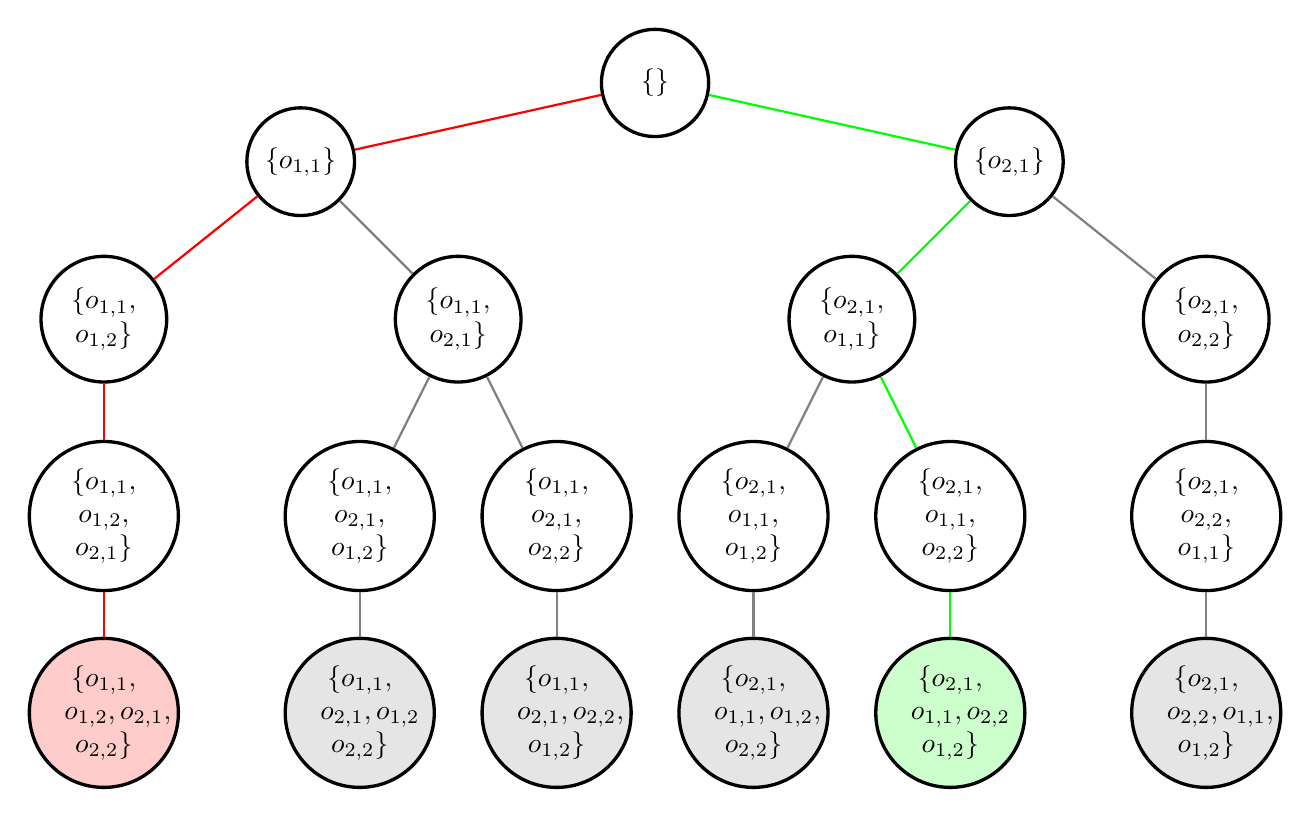
\begin{tikzpicture}[
    node/.style={circle, draw, minimum size=10mm, very thick, text width=10mm, align=center},
    message/.style={->, >=Stealth, thick, bend left=20}
]

% Nodo centrale
\node[node] (center) at (0,4) {$\{\}$};

% Nodi vicini
\node[node] (n1) at (-4.5,3) {$\{o_{1,1}\}$};
\node[node] (n2) at (4.5,3) {$\{o_{2,1}\}$};

% Edges del grafo
\draw[thick, red] (center) -- (n1);
\draw[thick, green] (center) -- (n2);

\node[node] (n5) at (-7, 1) {$\{o_{1,1},$\\$o_{1,2}\}$};
\node[node] (n10) at (-2.5, 1) {$\{o_{1,1},$\\$o_{2,1}\}$};
\node[node] (n8) at (2.5, 1) {$\{o_{2,1},$\\$o_{1,1}\}$};
\node[node] (n7) at (7, 1) {$\{o_{2,1},$\\$o_{2,2}\}$};

\node[node] (n100) at (-7, -1.5) {$\{o_{1,1},$\\$o_{1,2},$\\$o_{2,1}\}$};
\node[node, fill=red!20] (n101) at (-7, -4) {$\{o_{1,1},$\\$o_{1,2},o_{2,1},$\\$o_{2,2}\}$};

\node[node] (n102) at (-3.75, -1.5) {$\{o_{1,1},$\\$o_{2,1},$\\$o_{1,2}\}$};
\node[node] (n103) at (-1.25, -1.5) {$\{o_{1,1},$\\$o_{2,1},$\\$o_{2,2}\}$};

\node[node, fill=gray!20] (n108) at (-3.75, -4) {$\{o_{1,1},$\\$o_{2,1},o_{1,2}$\\$o_{2,2}\}$};
\node[node, fill=gray!20] (n109) at (-1.25, -4) {$\{o_{1,1},$\\$o_{2,1},o_{2,2},$\\$o_{1,2}\}$};

\node[node] (n104) at (1.25, -1.5) {$\{o_{2,1},$\\$o_{1,1},$\\$o_{1,2}\}$};
\node[node] (n105) at (3.75, -1.5) {$\{o_{2,1},$\\$o_{1,1},$\\$o_{2,2}\}$};

\node[node, fill=green!20] (n110) at (3.75, -4) {$\{o_{2,1},$\\$o_{1,1},o_{2,2}$\\$o_{1,2}\}$};
\node[node, fill=gray!20] (n111) at (1.25, -4) {$\{o_{2,1},$\\$o_{1,1},o_{1,2},$\\$o_{2,2}\}$};

\node[node] (n106) at (7, -1.5) {$\{o_{2,1},$\\$o_{2,2},$\\$o_{1,1}\}$};
\node[node, fill=gray!20] (n107) at (7, -4) {$\{o_{2,1},$\\$o_{2,2},o_{1,1},$\\$o_{1,2}\}$};

\draw[thick, gray] (n1) -- (n10);
\draw[thick, red] (n1) -- (n5);
\draw[thick, green] (n8) -- (n2);
\draw[thick, gray] (n7) -- (n2);
\draw[thick, red] (n5) -- (n100);
\draw[thick, red] (n100) -- (n101);
\draw[thick, gray] (n10) -- (n102);
\draw[thick, gray] (n10) -- (n103);
\draw[thick, gray] (n8) -- (n104);
\draw[thick, green] (n8) -- (n105);
\draw[thick, gray] (n7) -- (n106);
\draw[thick, gray] (n106) -- (n107);
\draw[thick, gray] (n102) -- (n108);
\draw[thick, gray] (n103) -- (n109);
\draw[thick, gray] (n104) -- (n111);
\draw[thick, green] (n105) -- (n110);

\end{tikzpicture}
\caption{A tree representing all the possible schedules for a $2\times2$ JSP. The gray nodes are the complete schedules. The red node represent the schedule obtained through the SJF euristic (not optimal). The green node represent the optimal schedule.}
\label{fig:Tree_schedule}
\end{figure}

In the example shown before (\ref{fig:Tree_schedule}), the approach using the euristic called Shortest Job First (SJF) would give a schedule that isn't optimal, exactly this one:
$$[o_{1,1}, o_{1,2}, o_{2,1}, o_{2,2}]$$
(the schedule obtained through this euristic is the red node in the tree, it is obtained through the red path). This schedule is going to take 9 time steps to finish.\\
The optimal schdeule is instead:
$$[o_{2,1}, o_{1,1}, o_{1,2}, o_{2,2}]$$
(the schedule is shown represented in the tree as the green node, obtained through the green path). This schedule is going to take 8 time steps to finish, making it the most efficient one.
This shows how the JSP is difficult to solve optimally, technically for be sure to find the optimal schedule there is the need to search through all the possible combinations and this is not feasible for big problems.


\section{Thesis structure}
%In a paper of the Department of Computer Science of the University of Turin \cite{LION17}, they approach the creation of a good schedule by using a neural network that will be described in another section. The aim of this thesis is to try modify the way the problem was seen, making the input a graph to express the problem in a more natural way.\\
%I decided to modify only the encoding part and for now leave the decoder with the same layers as they imagined. The problem is approached with a deep reinforcement technique.\\
The aim of this thesis is to implement a model based on the Graph Convolutional Networks (GCN) to find a very good solution to the Job Shop Problem (JSP) (not the best one since the problem is NP-hard). The graph model is inspired by the article of the Department of Computer Science of the University of Turin \cite{LION17}. The aim of this thesis is to try modify the way the problem was seen, making the input a graph to express the problem in a more natural way.\\
The only section that is modified from the original model is the encoder, the decoder has the same structure and the problem is approached with a deep reinforcement technique.\\
The code is publicly available on GitHub\cite{GitHub}.
\begin{itemize}
    \item \textbf{Chapter 2:} a brief recap on how the different arguments explored in this thesis works, starting from the GNN and reaching up to the specific deep reinforcement technique used in the original article and also used in this new implementation.
    \item \textbf{Chapter 3:} an explanation on how the data are obtained, how the data are modified in a graph structure and how the models are implemented, the one of the paper and the one modified.
    \item \textbf{Chapter 4:} an explanation and a discussion on the results of the model with a matrix representation and the modified one.
\end{itemize}




\chapter{Background}
In this section there will be a very brief explanation on how the different parts of the model work and how it works the idea behind the reinforcement learning technique used.\\
More specifically, the Graph Convolutional Network (GCN) is used in the encoder, the Long-Short Term Memory (LSTM) and the Pointer Network are used in the decoder.
\section{Graph Convolutional Network (GCN)}
The Graph Convolutional Network (GCN) is a specific type of neural network that takes in input a graph instead of a tensor, as in basic neural networks. GCNs were introduced by Kipf and Welling \cite{kipf2017semi}.\\
We will mainly use convolutional layers in order to pass information about the operations. The convolution in this case is very different from the convolution in the Convolutional Neural Networks (CNN), in the CNN the convolution is a weighted sum of the values in a $k\times k$ grid (applying a kernel), the GCN instead performs these steps for every node of the graph:
\begin{itemize}
    \item selects all the different nodes connected to the node that are working on
    \item aggregates all the nodes.
    \item multiplies with the weight matrix, apply a transformation.
    \item applies an activator function (ex. ReLU).
\end{itemize}

This operation can be made really fast by doing some matrix multiplications:
$$H^{(l+1)}=\sigma(\tilde{D}^{-{1\over2}}\tilde{A}\tilde{D}^{-{1\over2}}H^{(l)}W^{(l)})$$
where:
\begin{itemize}
    \item $H^{(l)}$ is the matrix of the features at layer $l$, where each row represents the features of a node.
    \item $W^{(l)}$ is the weight matrix at layer $l$.
    \item $\tilde{A}=A+I$ is the adjacency matrix of the graph with added self-loops (I is the identity matrix).
    \item $\tilde{D}$ is the degree matrix of $\tilde{A}$.
    \item $\sigma$ is an activation function, for example ReLU.
\end{itemize}

The normalization term $\tilde{D}^{-{1\over2}}\tilde{A}\tilde{D}^{-{1\over2}}$ prevents high-degree nodes from dominating the aggregation and ensures numerical stability.
With this approach after one layer a node combines its features and the ones of the nodes directly connected to it, its neighbors. In the second layer a node will have the collection of features that it, its neighbors and the neighbors of the neighbors and so on.\\
There is a problem with this approach, it's called oversmoothing: when you apply this convolution too many times the features are too similar and there is a risk to lose local information.

\begin{figure}[h]
\centering
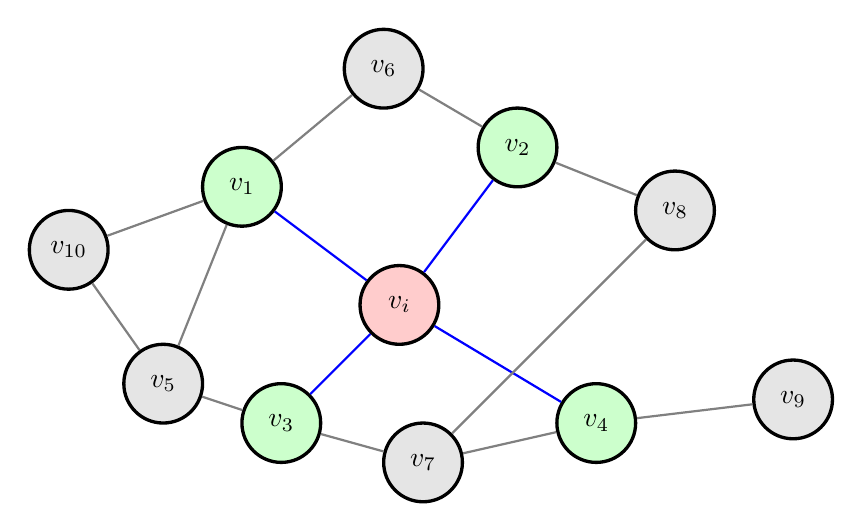
\begin{tikzpicture}[
    node/.style={circle, draw, minimum size=10mm, very thick},
    message/.style={->, >=Stealth, thick, bend left=20}
]

% Nodo centrale
\node[node, fill=red!20] (center) at (0,0) {$v_i$};

% Nodi vicini
\node[node, fill=green!20] (n1) at (-2,1.5) {$v_1$};
\node[node, fill=green!20] (n2) at (1.5,2) {$v_2$};
\node[node, fill=green!20] (n3) at (-1.5,-1.5) {$v_3$};
\node[node, fill=green!20] (n4) at (2.5,-1.5) {$v_4$};

% Edges del grafo
\draw[thick, blue] (center) -- (n1);
\draw[thick, blue] (center) -- (n2);
\draw[thick, blue] (center) -- (n3);
\draw[thick, blue] (center) -- (n4);

\node[node, fill=gray!20] (n5) at (-3, -1) {$v_5$};
\node[node, fill=gray!20] (n6) at (-0.2, 3) {$v_6$};
\node[node, fill=gray!20] (n7) at (0.3, -2) {$v_7$};
\node[node, fill=gray!20] (n8) at (3.5, 1.2) {$v_8$};
\node[node, fill=gray!20] (n9) at (5, -1.2) {$v_9$};
\node[node, fill=gray!20] (n10) at (-4.2, 0.7) {$v_{10}$};

\draw[thick, gray] (n1) -- (n10);
\draw[thick, gray] (n3) -- (n5);
\draw[thick, gray] (n1) -- (n5);
\draw[thick, gray] (n10) -- (n5);
\draw[thick, gray] (n1) -- (n6);
\draw[thick, gray] (n6) -- (n2);
\draw[thick, gray] (n8) -- (n2);
\draw[thick, gray] (n7) -- (n8);
\draw[thick, gray] (n7) -- (n4);
\draw[thick, gray] (n7) -- (n3);
\draw[thick, gray] (n4) -- (n9);

\end{tikzpicture}
\caption{Message passing in a GCN, the node takes the information from the neighbors.}
\label{fig:message_passing}
\end{figure}

\section{Long-Short Term Memory (LSTM)}
The Long-Short Term Memory (LSTM) is a specific type of recurrent neural network that helps to solve the problem of the vanishing/exploding gradient, a very well known problem in the Recurrent Neural Networks (RNN) where the backpropagation of the gradient vanishes/explode because of the recursive layers. LSTMs were introduced by Hochreiter and Schmidhuber \cite{hochreiter1997lstm}. The innovation is that this kind of neurons have a long-term memory, a short-term memory and their relations.\\
This kind of layer has 3 different gates: input gate, forget gate and output gate.
\begin{itemize}
    \item Input gate: it represents the percentage of information that is going to be remembered in the long-term memory, so 0 is nothing and 1 is everything.
    \item Forget gate: it represents how important is should be considered of the long-term memory, how important should be considered.
    \item Output gate: Decide how to implement the long-term memory, the short-term memory and the input, at the end sends the final value and that final value is going to be re-used for the short-term memory for the next value.
\end{itemize}

There are 3 values at input that represent: the input, the information in that exact moment, the memory of the previous information (like a short-term memory), and a representation of all the previous information (like a long-term memory). These values are usually represented as $x_t$, $h_t$ and $c_t$.\\
To decide the values for the different gates we are going to multiply the 3 values $x_t$, $h_{t-1}$ and $c_{t-1}$ (there is t-1 obviously because we take the memory of previous state) by a value between 0 and 1 which can be easily obtained with a sigmoid function. The input of the sigmoid function is going to be $x_t$ and $h_{t-1}$ and it makes sense since the weight of the long-term memory depends on the short-term memory and the information that is inserted in that moment.\\
\begin{itemize}
    \item The forget gate is very simple: it is just the sigmoid function and we are going to multiply the output of sigmoid function with the long-term memory $c_{t-1}$, it represents how much information should be used from the old data, how much are important.
    \item The input gate is a little bit more complicated: there is a sigmoid function but this time does not multiply the long-term memory, it is multiplied with a hyperbolic tangent (again the input are $x_t$ and $h_{t-1}$) and then this multiplication is summed with the long-term memory. This operation is like an update of the long-term memory with the new information.
    \item The final gate, the output gate, takes again a sigmoid function of the 2 values but now it multiplies with the hyperbolic tangent of the long-term memory $c_t$. The result of this operation is the new short-term memory $h_t$ and the output of the layer.
\end{itemize}

\begin{figure}[htp]
    \centering
    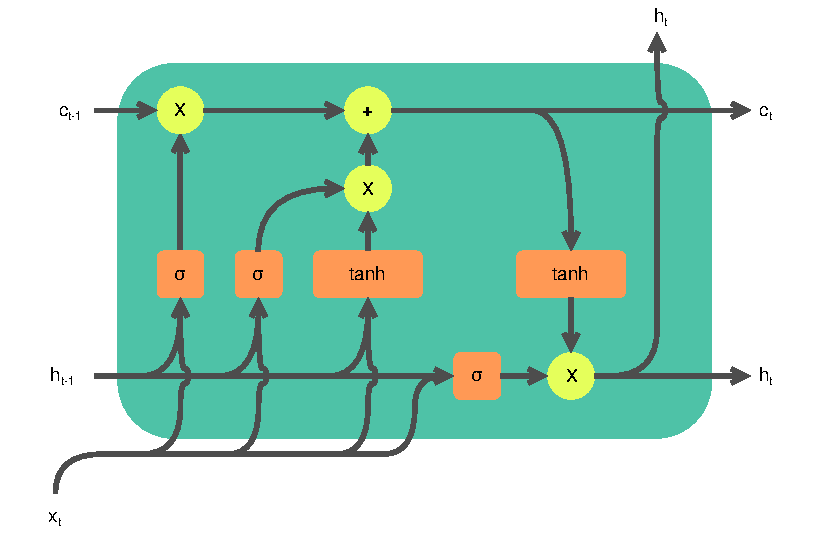
\includegraphics[width=8cm]{LSTM_cell.pdf}
    \caption{Image of a LSTM layer}
    \label{fig:LSTM layer}
\end{figure}

To summarize, at the beginning there is the forget gate, after there is the input gate and here we obtain the new updated long-term memory $c_t$, the last one is the output gate and here are used $x_t$, $h_{t-1}$ and $c_t$ to calculate $h_t$ (that is the output of the node too).\\
This kind of layer is important to decide which operation we are going to do right now, because it will evaluate the different operation by taking consideration of the previous operations, in the short and in the long time. 

\section{Pointer network}

A pointer network is a specific type of neural network where the output is an element of the input, for example if there is a set of elements $\{1,2,3,4,5\}$ then the Pointer network is going to give an element of the input as output, for example it could be 4. Pointer Networks were introduced in \cite{vinyals2015pointer}.\\
In this case it is particularly useful because the neural network can decide which operation to choose in that exact moment and we can do it with whatever dimension of the set we want. To do this we are going to repeat the LSTM layer and the pointer mechanism $n\times m$ times.\\
The main idea of the pointer network is centered in an attention mechanism, in this case also called as a pointer mechanism:
\[\alpha_{t,i}=\mathrm{softmax}(v^T\tanh(W_1h_i+W_2s_t))\]
The most critical part to understand is that $h_i$ is a vector that codifies the information about an input. This means that there will be $n$ vectors $h_i$ where $n$ is the number of inputs.\\
This mechanism takes a weighted linear sum of the encoding and the decoding (respectively $h_i$ and $s_t$) and applies a non-linear transformation, $tanh$, to obtain a value between -1 and 1. To transform this vector into a number we multiply it by the transpose of a vector $v$. At the end a softmax is applied so the final values are between 0 and 1 with a higher value if the value before was high with respect to the other values.\\
The result of this operation is a vector of values: $\alpha=[\alpha_1,...,\alpha_n]$ where $\sum_{i=1}^n\alpha_i=1$ (because of the softmax distribution operation).\\
In the training we are going to select a value randomly according to the distribution but when we are testing or executing the program normally we are not going to choose randomly but the highest value.

\section{Deep Reinforcement Learning}
The paper decided to apply the reinforcement learning to train the neural network, a policy gradient method.\\
The policy gradient method is focused to learn the parameters $\theta$ for optimizing a stochastic policy $\pi_\theta$ (approximated by the neural network) \cite{williams1992simple}.. The policy takes as argument a state and produce a probability distribution over the possibles actions, and by following the definition of distribution we should have that: \[ \sum_{a\in Act} \pi(a|s) = 1 \]
We take those action and by doing this we create an episode $\tau$, more formally: a sequence of states and actions ($s_0, a_0, s_1, a_1,...,s_H$) with a return value $R(\tau)$ that is calculated in this way:
\[ \sum_{i=0}^{H} R(s_i, a_i, s_{i+1})\]
Also known a finite Horizon Undiscounted Return.\\
A very important part is the mathematical formula to calculate the probability of going to a certain episode given a fixed policy, given by this formula:
\[P_\theta(\tau) = \rho(s_0)\prod_{t=0}^{H}T(s_{t+1}|s_t, a_t)\pi_\theta(a_t|s_t)\]
Where $\rho(s_0)$ is the probability to have $s_0$ as first state.
Our goal obviously is to have the biggest return as possible, so we are doing a maximization over the expected value of the return:
\[\max_\theta J(\pi_\theta)\quad \textrm{where}\quad J(\pi_\theta) = \mathbb{E}_{\tau \sim \pi_\theta}\left[R(\tau) \right]\]

We can achieve a good good policy by doing a policy ascent, to do so we need to evaluate $\nabla_\theta J(\pi_\theta)$, the gradient of the expected value of the return of a episode made by following a policy, also known as the policy gradient. It can be shown that the policy gradient is:
\[\nabla_\theta J(\pi_\theta) = \mathbb{E}_{\tau \sim \pi_\theta}\left[\sum_{t=0}^{H}\nabla_\theta \textrm{log}\pi_\theta(a_t|s_t)R(\tau)\right]\]

This is also known as Vanilla policy gradient.
The problem is that this method suffers from high variance, given from the fact that $\nabla_\theta J(\pi_\theta)$ is unbiased. To improve we can add into the formula the component of the baseline, a term that depends only from the current state. The formula becomes:
\[\nabla_\theta J(\pi_\theta) = \mathbb{E}_{\tau \sim \pi_\theta}\left[\sum_{t=0}^{H}\nabla_\theta \textrm{log}\pi_\theta(a_t|s_t)\left(\sum_{i=t}^{H}R(s_i, a_i, s_{i+1}) - b(s_t)\right)\right]\]
\chapter{Methods applied}
\section{Data}
The easiest way to acquire the data is by randomly generating them, in this way it's able to generate many different instances with different numbers of jobs and machines.\\
In these experiments the models are trained only on a $6\times6$ JSP, an adequate measure. The decision is also based on making easier the training for batches because otherwise the risk would be to have a batch made of different elements and this would make the GCN raise an exception (there is the possibility to train batches of same dimensions with the dimensions in the batches is different, but in the result section there would be a part where is discussed how this new implementation is able to understand a rule based on any number of $n$ jobs and $m$ machines).
\subsection{Representation of the data in the article}
In the paper, the problem is represented in the easiest possible way: a matrix. The matrix has 4 columns and $n\times m$ rows, each row represents a single operation and it has those feature (in the exact order): the id number of the job $i$ (so from which job comes that operation), the position of the operation in that job $j$, which machine is required for that operation $M_{i,j}$ and how much time it takes to execute that operation $p_{i,j}$.\\
So a row is represent like this:
\[o_{i,j} = [i, j, M_{i,j}, p_{i,j}]\]
And the entire JSP can be represented as: 
\[
    S^{seq} = \begin{bmatrix}
           o_{0,0} \\
           o_{0,1} \\
           \vdots \\
           o_{(n-1),(m-1)}
         \end{bmatrix}
\]
In the paper, the goal is to obtain a sequence of instructions where the makespan is as little as possible, so by thinking that at the end the operations will be the same but in a different order the solution can be written as: 
\[L^{seq}=PS^{seq}\]
where P is a permutation matrix and $L^{seq}$ is a feasible solution.

\subsection{Representation of data in the graph model}
The data in this case are represented in a different way, which may better represent to represent the data in a more accurate way: a graph\cite{Vesselinova2020}.\\
The graph is structured with 2 category of nodes: operation nodes and machine nodes. The operation node represents a single operation instead a machine node represents a single machine.\\
The nodes are connected in this way:
\begin{itemize}
    \item an operation node is connected with another operation node if one is the next one of the other. The connection is unidirectional, from the operation that comes before to the next one.
    \item an operation node is connected with a machine node if that operation is executed by that machine. This time the connection is bidirectional
\end{itemize}
Every node has 4 features, but the meaning of the features is different between the 2 nodes:
\begin{itemize}
    \item in an operation node, the features represent: at which step the operation is in a job (the parameter before called $j$), the processing time but normalized, the number of operations that are left and the typology of the node (1 if the node is an operation node and 0 if the node is a machine node)
    \item in a machine node, the features represent: -1 (a value that is useless and impossible for the operation node, so it's a one more check to see if it's a machine node), the total workload in a machine (but it's "normalized" by dividing it with 1000), number of operations that a machine has to execute (it will be $n$, the number of jobs because it's a JSP) and like in the operation node a variable to understand the typology of the node (1 if the node is an operation node and 0 if the node is a machine node).
\end{itemize}

\begin{figure}[h]
\centering
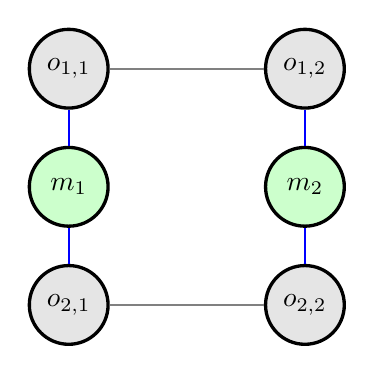
\begin{tikzpicture}[
    node/.style={circle, draw, minimum size=10mm, very thick},
    message/.style={->, >=Stealth, thick, bend left=20}
]

% Nodo centrale

% Nodi vicini
\node[node, fill=green!20] (n1) at (-3,1.5) {$m_1$};
\node[node, fill=green!20] (n2) at (0,1.5) {$m_2$};

\node[node, fill=gray!20] (n5) at (-3, 3) {$o_{1,1}$};
\node[node, fill=gray!20] (n6) at (0, 3) {$o_{1,2}$};
\node[node, fill=gray!20] (n8) at (-3, 0) {$o_{2,1}$};
\node[node, fill=gray!20] (n9) at (0, 0) {$o_{2,2}$};
\draw[thick, blue] (n5) -- (n1);
\draw[thick, blue] (n8) -- (n1);
\draw[thick, blue] (n6) -- (n2);
\draw[thick, blue] (n9) -- (n2);

\draw[thick, gray] (n5) -- (n6);
\draw[thick, gray] (n8) -- (n9);

\end{tikzpicture}
\caption{Example of a $2\times2$ JSP, the gray connections represent the connections between 2 operation nodes (and the are unilateral connection from $o_{i,j}$ to $o_{i,j+1}$ if there exists such operation) and the blue connections represent the connection between a operation node and a machine node.}
\label{fig:graph_example}
\end{figure}

\section{Architecture of the matrix model}
The matrix model is divided in 2 parts, an encoder and a decoder \cite{LION17}. The encoder is a self-attention-based model where the input is a tridimensional tensor $U\in\mathbb{R}^{N\times(mn)\times4}$ where $m$ and $n$ are the number of machines and the number of nodes, 4 are the features of an operation and $N$ is the batch size.
\subsection{Encoder}
The first operation of the encoder is to divide the tensor between the first 2 features (the id of the job and the position in that job of the operation) and the other 2 features (which machine should execute that operation and how much time it should take). In each division it's applied a batch normalization and then a linear layer, also known as a dense layer (the most basic type of operation in a neural network). After this transformations the 2 divisions are summed element by element, it's done another batch normalization and another linear layer (after each linear layer is applied a ReLU as usual).\\
For the last part it's applied a $l$ multi-head attention layer (they consider $l=3$), so the final output of the encoder is going to be $H\in\mathbb{R}^{N\times(nm)\times d_h}$ with each row $h_k\in\mathbb{R}^{d_h}$ that are going to be used for the decoder.

\begin{figure}[htp]
    \centering
    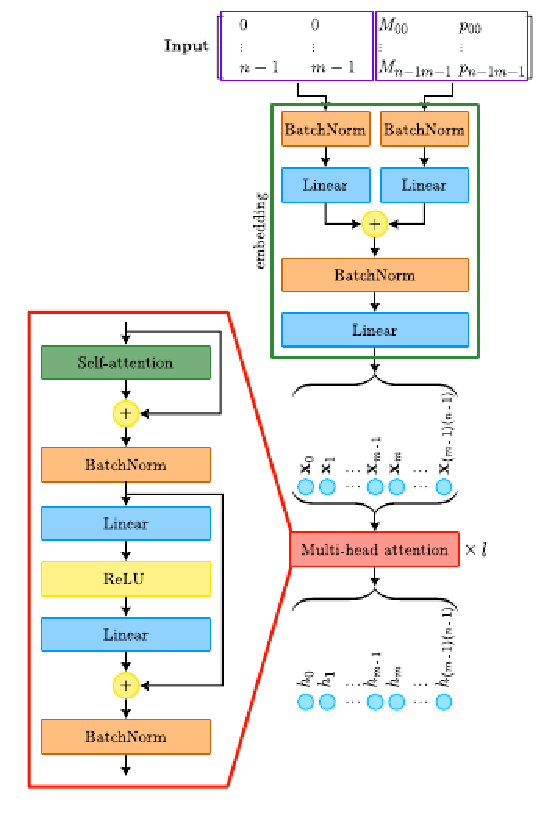
\includegraphics[width=8cm]{Encoder_paper.pdf}
    \caption{Image representing the encoder of the paper}
    \label{fig:Paper encoder}
\end{figure}

\subsection{Decoder}
The decoder has a LSTM layer, very useful in this case because a precedent decision (very far away or not) vastly impact the next choice, after this layer is applied the attention mechanism to make a probability of which element to choose, generating the policy $\pi_\theta$.\\
The problem is this kind of operation generate a probability over all the values of input, and this is not a good solution because there is the possibility to choose a operation already been chosen or choose a operation that should be taken in the future (rules of the JSP). To solve this problem before doing the softmax is going to be applied a mask that would set at $-\infty$ the values so when the softmax distribution is going to be applied the value will be $0$. So the final policy distribution will be:
\[\pi_\theta (o_t'|o_0',o_1',\dots,o_{t-1}',S^{seq})=\mathrm{softmax}(\mathrm{mask}(u^t|o_0',o_1',\dots,o_{t-1}'))\]
where $u^t$ is the score calculated by the attention mechanism at the $t$ step, mask is the masking procedure applied to obtain possibilities over only operations that are "legals".
The policy distribution is obtained $n\times m$ times, so the entire procedure is going to be applied this many times.

\begin{figure}[htp]
    \centering
    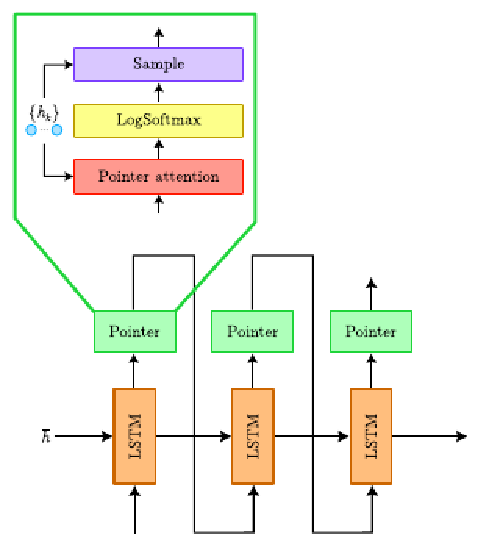
\includegraphics[width=8cm]{Decoder.pdf}
    \caption{Image representing the decoder of the paper}
    \label{fig:Decoder}
\end{figure}

\subsubsection{Masks}

As mentioned in the previous section, it is necessary to apply a mask. A mask is an array of ones and zeros where in this case shows the "legal" possibilities, so if there is False in the position $i$, then the operation $o_i$ is possible to be selected (because we are going to change values only where the index are True). This is particularly useful because we need to be able to set some values such that the probability of making a wrong choice is $0$, to make so all the impossible decisions are going to be set at $-\infty$, because when it's applied the softmax the value is set to $0$, it can be seen in the formula:

\[\mathrm{softmax}(z)_i = \frac{e^{z_i}}{\sum_{j=1}^N e^{z_j}}\]

It is easy to see that the $\lim_{z\rightarrow -\infty}e^z=0$, making the choice impossible to pick.\\
Are two kinds of masks are applied to set the values at $-\infty$: one about the sequence of the operations and one about if the operation is already scheduled or not (they are going to be called $M^{mask}$ and $M^{sched}$).
\begin{itemize}
    \item $M^{mask}$: given the instance of a batch $k$ and the index of the operation of the $i^{th}$ job $l$ (also written as $p=i\cdot m + l$), the value $M^{mask}_{kp}$ will be true if $l>j$, where $j$ is the index of the last operation executed by the $i^{th}$ job. This mask is needed to follow the normal flow of the operations, in the right order.
    \item $M^{sched}$: given the instance of a batch $k$ and the index of the $i^{th}$ job $l$ (also written as $p=i\cdot m + l$), the value $M^{sched}_{kp}$ will be true if the the $j^{th}$ operation of the $i^{th}$ job has already been scheduled.
\end{itemize}

The union of those 2 matrices will give in the slots with the value False the operations that it is possible to use (or if it's seen in the other way, the slots where the value are false are the ones that can't be done at least for the moment.

\section{Architecture of the graph model}
In the graph model the encoder is going to be modified and leave the decoder the same as the one in the paper.\\
The new encoder is based on a graph representation of the data, so it will be a GNN, more specifically a GCN. The model start with a GCN layer and and then it has 2 blocks of layers made as: Layer Normalization, ReLU activators and  Graph's Convolution. It utilizes only a total of 3 graph convolutional layers to prevent the risk of oversmoothing.\\
To apply the decoder of the paper the output should be a tensor $H\in\mathbb{R}^{N\times(nm)\times d_h}$, so the operation made to get the matrix is a filter of the nodes where are obtained only the operation nodes and then translate the graph into the tensor. 

\begin{figure}[htp]
    \centering
    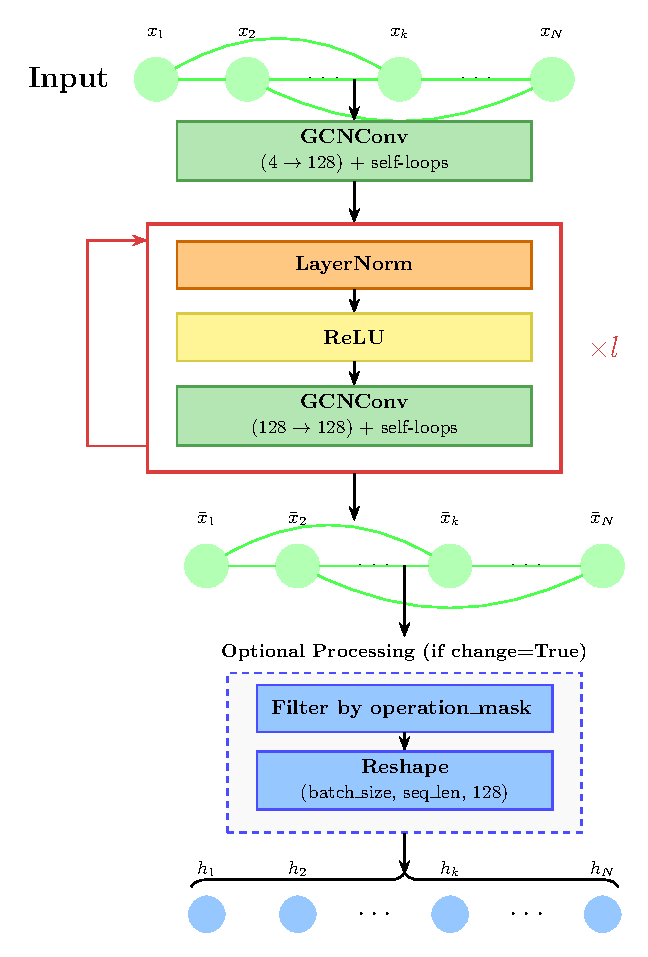
\includegraphics[width=8cm]{GCN_Encoder.pdf}
    \caption{Image representing the encoder of the new implementation where there is at first a GCN Layer and then an arbitrary number of LayerNorm, Relu and GCN Layers that are repeated in this order, in this case $l=2$.}
    \label{fig:GCN Encoder}
\end{figure}

\subsection{Transformation from graph to matrix}
To apply the decoder of the paper it's necessary to transform the graph representation into a matrix representation.
The matrix on the paper is of dimension $N\times (nm)\times d_h$ (where $N$ is the batch size, $n$ the number of jobs, $m$ the number of machines and $d_h$ the dimension of the features after the encoding).\\
The graph at the end of the encoder has $(nm)+m$ nodes because there are $nm$ operation nodes and $m$ machine nodes where in each node there is a vector of dimension $d_h$. If we don't consider the $m$ nodes that represent the machines then we have $nm$ nodes with a vector of features $d_h$, so it's easy to create the matrix representation just by taking the features of the operation nodes and stacking them in the right order.\\
Since every the models were only trained on the $6\times6$ JSP, the matrix can be created easily in this way:

\begin{lstlisting}[caption={Transformation from graph to matrx}, label={lst:fib}]
if batch_size is not None and seq_len is not None and change:
    if operation_mask is not None:
        # Filtra solo le feature dei nodi delle operazioni
        x = x[operation_mask]
        x = x.view(batch_size, seq_len, self.d_model)
            
return x
\end{lstlisting}

\section{Training of the neural networks}

The models were trained using a policy gradient method (with an ADAM optimizer): 
\[\nabla_\theta L(\pi_\theta) = \mathbb{E}\left[(C_{max}(L^{seq})-b(S^{seq}))\nabla_\theta \mathrm{log}P_\theta(L^{seq}|S^{seq})\right]\]
where $P_\theta(L^{seq}|S^{seq})=\prod_{t=0}^{n\cdot m - 1}\pi_\theta(o_t'|o_0', o_1',...,o_{t-1}', S^{seq})$ so it's the probability of getting the solution $L^{seq}$ following the policy $\pi_\theta$ and given a problem $S^{seq}$. After each epoch, the baseline is updated with the optimized policy's weights only if the policy is statistically better. This update ensures that we are training our policy with the the best policy found so far.\\
The models were trained 150 epochs, with 10 thousand elements as a training set and a thousand elements for validation and test set. They were trained in CPU and not GPU because the model doesn't have an excessive amount of variables to calculate, it takes more time to send the data into the GPU than calculating everything in the CPU.
\begin{center}
\begin{tabular}{|c | c |} 
 \hline
 Parameter & Value \\  
 \hline
 Hidden dimension & 128 \\ 
 \hline
 number of GCN layers & 3 \\
 \hline
 Learning rate & 0.0001 \\
 \hline
 Learning rate decay & None \\
 \hline
 Batch size & 512 \\
 \hline
 Training epochs & 150 \\
 \hline
 Training set size & 10,000 \\
 \hline
 Validation/test set size & 1,000 \\
 \hline
 CPU/GPU & CPU \\
 \hline
 CPU & Intel Core i7-6700 \\
 \hline
 Time for epoch & $\sim$ 90 sec \\
 \hline
\end{tabular}
\end{center}

It took the same amount of time to train both the models, around 90 seconds for each epoch.

\chapter{Results and comparison}

These models where trained only using a $6\times6$ JSP, in the paper the matrix model was trained with different settings to make the neural network understand how to solve the problem using different numbers of $n$ jobs and $m$ machines.\\
In this work the models were trained with only the $6\times6$ JSP to test an hypothesis: if a graph representation and so a GNN as an encoder is able to make the neural network understand the problem with a different number of $n$ jobs and $m$ machines.\\
The hidden dimension $d_h$ was set to 128 for both the models, the learning rate was set to 0.0001 without any decay and the batch size was set to 512.

\section{$\mathbf{6\times6}$ JSP}

The matrix model is making on average a policy where the result is just 23\% more than the actual best solution. The model with the GCN encoder instead gives a solution that is only 19\% more than the actual best solution.\\
The models reached an equilibrium at around 25-30 epochs (both of them), we can notice that the graph representation reaches a better result from the beginning, so it's without any doubt that the GCN encoder is able to understand the dynamic of the problem in a more accurate way than the matrix representation.

\begin{figure}[htp]
    \centering
    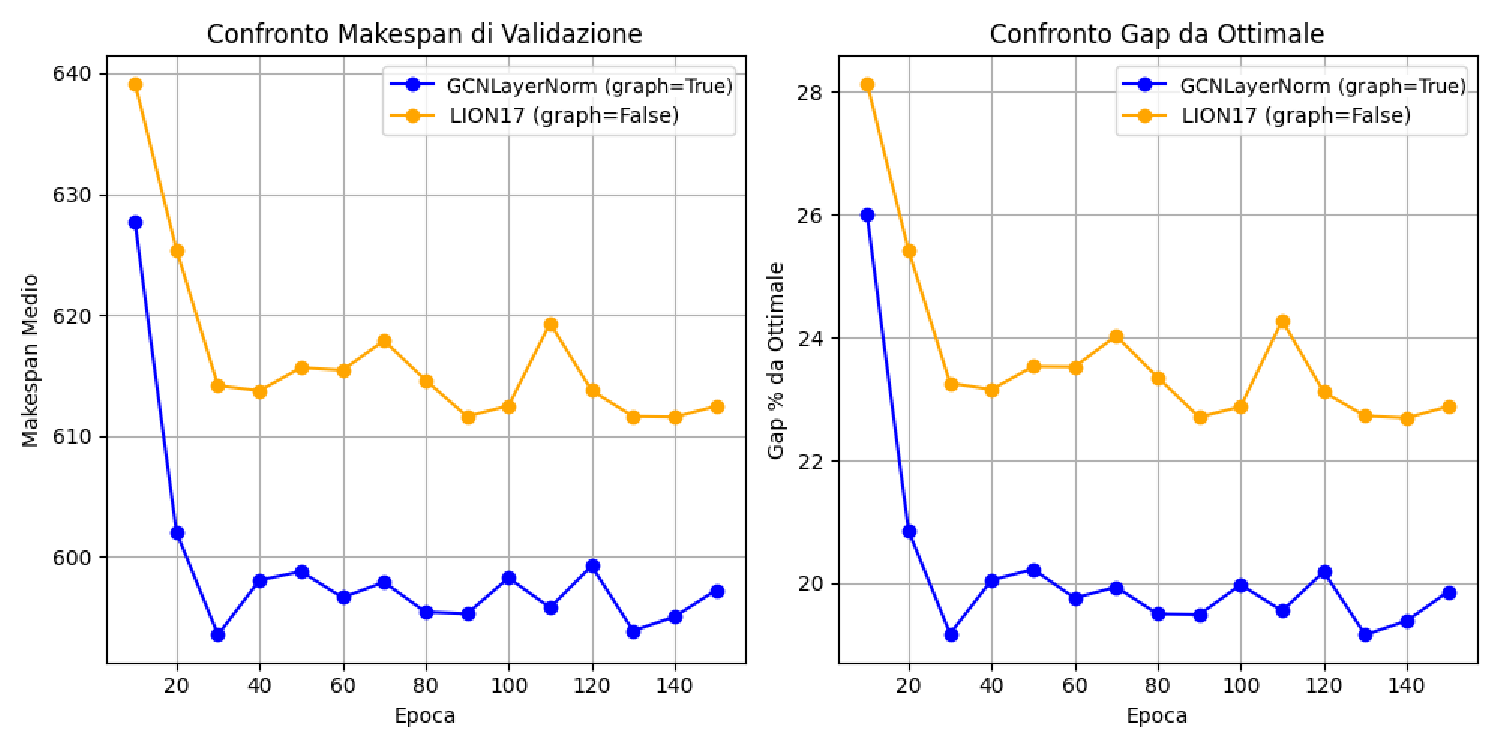
\includegraphics[width=10cm]{performance_comparison_LION_LayerNorm_6x6.pdf}
    \caption{Image representing the results of the validation test on the models on the $6\times6$ JSP.}
    \label{fig:6x6 JSP}
\end{figure}

This implies that the graph representation is able to express the problem and its characteristics in a more accurate way. The results in the image are obtained through a test set of 1000 elements.

\section{$\mathbf{n\times m}$ JSP}

After the results obtained through the training of the model with only the $6\times6$ JSP both the models were tested with different sizes of the JSP, to see if at least one of them is able to understand the logic with different number of jobs and machines.\\
In the paper, the normal model was trained with different sizes problems, so it was reasonable to expect that the model wouldn't be able to understand this complicate feature on its own with only one kind of problem.\\
The only hope was the modified version with the graph, hoping that it was able to understand how it should work with, hoping that the graph is able to express some constraints in a different way such that it is easier to find a solution even if the number of connections and nodes vary. It was reasonable to think it because the model is just a message passing model, so it just make a weighted sum of the values in different nodes.\\

\begin{figure}[htp]
    \centering
    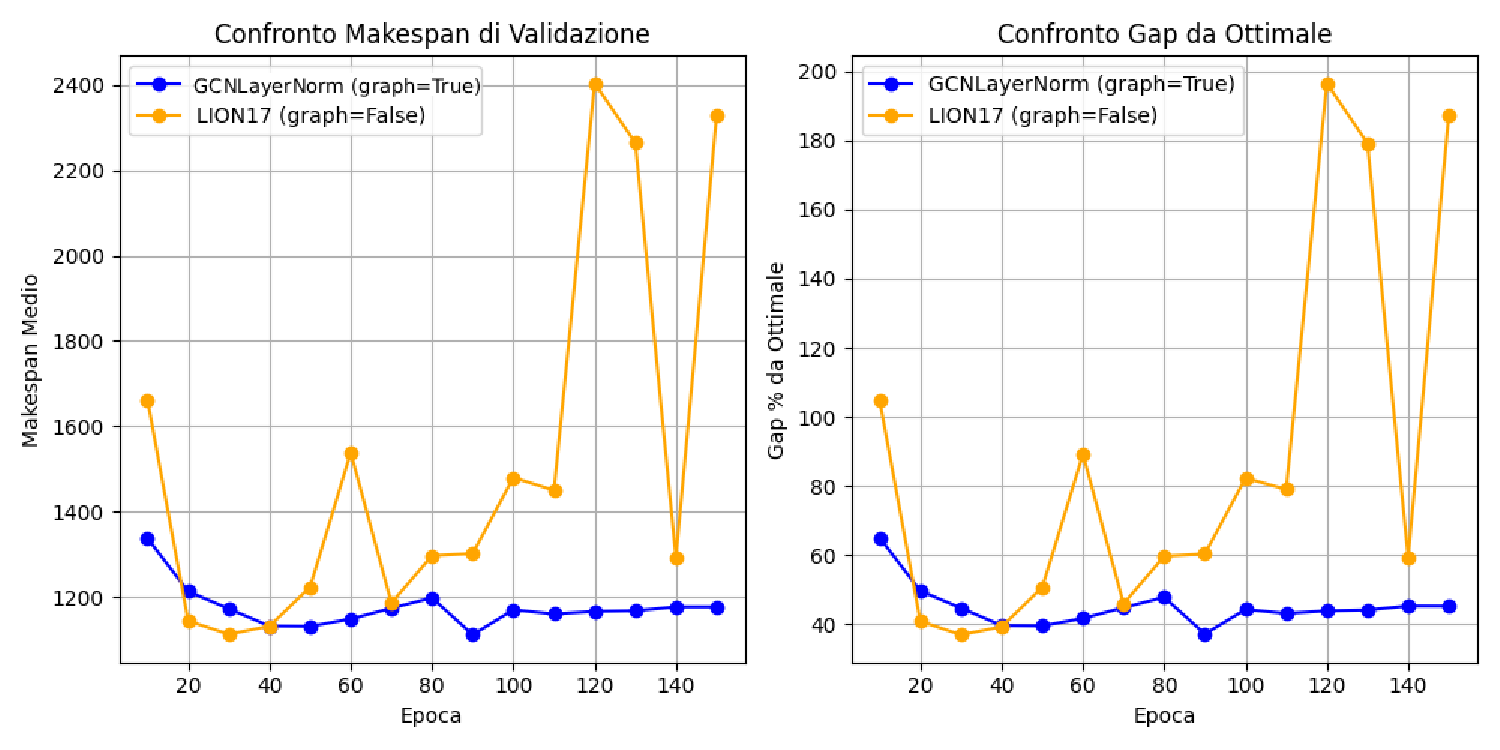
\includegraphics[width=10cm]{performance_comparison_LION_LayerNorm_10x10.pdf}
    \caption{Image representing the results of the validation test on the models on the $10\times10$ JSP.}
    \label{fig:10x10 JSP}
\end{figure}

In most cases it outperformed the matrix model, but at the beginning of the test it seemed as the matrix model was able to make a better schedule when the number of the number of the machines was higher than the number of the jobs, for example in the $5\times10$ JSP:

\begin{figure}[htp]
    \centering
    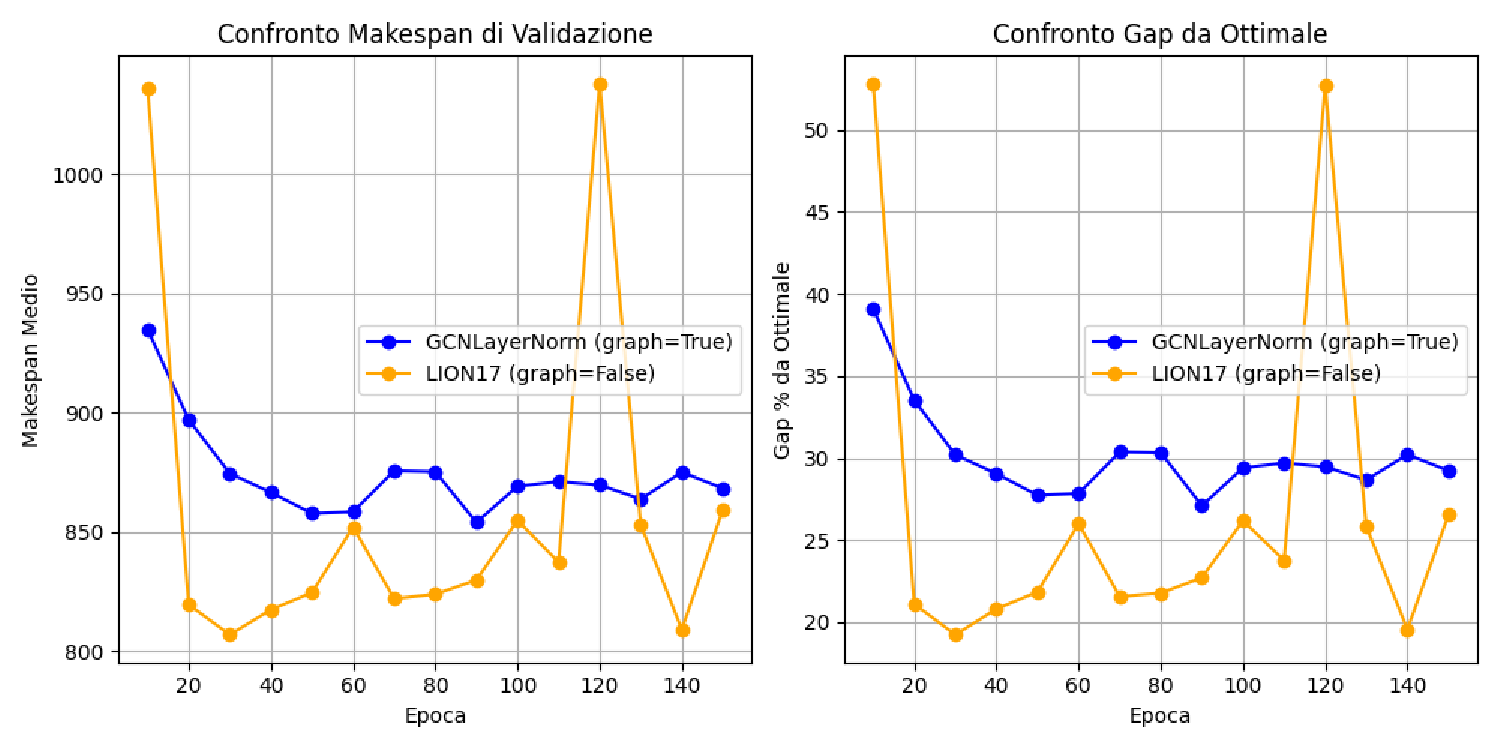
\includegraphics[width=10cm]{performance_comparison_LION_LayerNorm_5x10_3.pdf}
    \caption{Image representing the results of the validation test on the models on the $5\times10$ JSP.}
    \label{fig:5x10 JSP}
\end{figure}

This hypothesis is contradicted by the results on the $6\times15$ JSP where the model with the GCN encoder was able to make a better schedule than the other one.
\begin{figure}[htp]
    \centering
    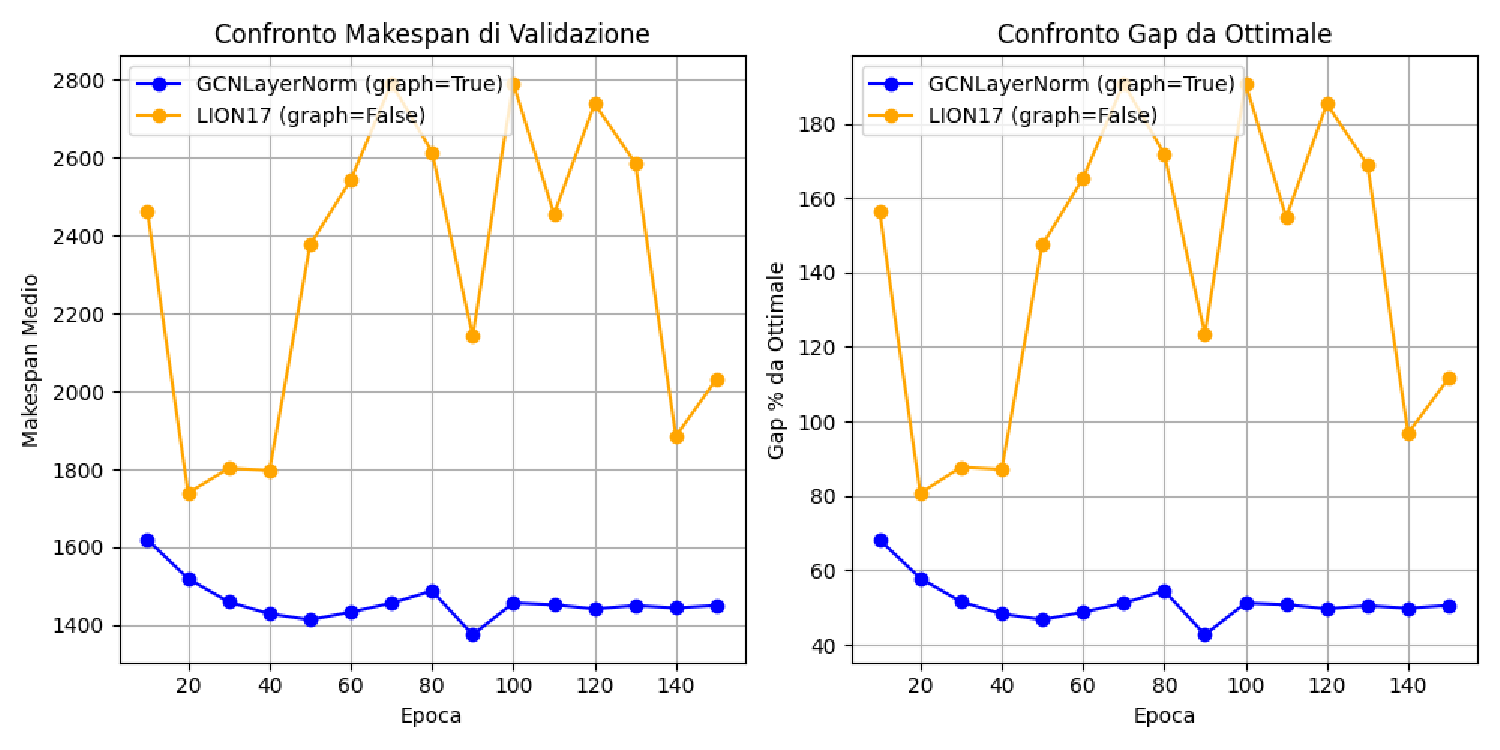
\includegraphics[width=10cm]{performance_comparison_LION_LayerNorm_6x15.pdf}
    \caption{Image representing the results of the validation test on the models on the $6\times15$ JSP.}
    \label{fig:6x15 JSP}
\end{figure}

There is a strong suggestion that the GCN encoder is able to understand the properties of the JSP through the graph representation for 3 reasons: due to the fact that the model outperforms most of the time the matrix model, the model doesn't spike randomly like it does the matrix model for all the tests different from the $6\times6$ problem and on all different sizes the GCN encoder model follows more or less the same path instead the matrix model follows more random paths, it doesn't seem to follow a pattern.
This fact is truly useful because it means that it is possible to train the model on samples of little dimensions and obtain a very good result that works very well even for very large size even if it has not ever seen one.\\
The fact that both models were trained only on $6\times6$ JSP is 
another element in favor of considering the baseline's superiority 
on the $5\times10$ problem as just an exception, because it doesn't make 
sense that it would generalize better to this specific configuration 
when it has only ever seen $6\times6$ JSP.\\
The models were tested with different sizes too, everything represented on a table, for simplicity
\begin{table}[htp]
\centering
\begin{tabular}{|c|c|c|c|}
\hline
JSP size & Perfect schedule & GCN encoder model & Paper model \\
\hline
$6\times6$ & 554 & 660 & 681 \\
\hline
& 520 & 588 & 686 \\
\hline
& 486 & 568 & 648 \\
\hline
& 527 & 621 & 630 \\
\hline
& 521 & 562 & 642 \\
\hline
$10\times10$ & 870 & 1258 & 2523 \\
\hline
& 889 & 1230 & 2189 \\
\hline
& 887 & 1338 & 2354 \\
\hline
& 802 & 1185 & 2521 \\
\hline
& 728 & 1161 & 2225 \\
\hline
$5\times10$ & 672 & 873 & 855 \\
\hline
& 675 & 1001 & 779 \\
\hline
& 744 & 911 & 808 \\
\hline
& 704 & 1037 & 758 \\
\hline
& 685 & 964 & 1043 \\
\hline
$6\times15$ & 918 & 1424 & 1992 \\
\hline
& 1056 & 1798 & 3006 \\
\hline
& 1004 & 1844 & 2767 \\
\hline
& 896 & 1118 & 1510 \\
\hline
& 974 & 1274 & 1960 \\
\hline
$10\times5$ & 622 & 765 & 778 \\
\hline
& 679 & 895 & 874 \\
\hline
& 576 & 722 & 746 \\
\hline
& 548 & 601 & 773 \\
\hline
& 613 & 676 & 900 \\
\hline
\end{tabular}
\caption{Makespan results for different Job Shop Problem (JSP) sizes.}
\label{tab:makespan_results}
\end{table}

\begin{table}[htp]
\centering
\begin{tabular}{|c|c|c|c|}
\hline
JSP size & Perfect schedule time & Time graph model & Time matrix model \\
\hline
$6\times6$ & 0.0219 s & 0.0381 s & 0.0212 s \\
\hline
& 0.0208 s & 0.0374 s & 0.0363 s \\
\hline
& 0.0390 s & 0.0445 s & 0.0285 s \\
\hline
& 0.0166 s & 0.0265 s & 0.0188 s \\
\hline
& 0.0213 s & 0.0167 s & 0.0162 s \\
\hline
$10\times10$ & 0.2927 s & 0.1150 s & 0.1236 s \\
\hline
& 0.2280 s & 0.2259 s & 0.2021 s \\
\hline
& 0.2588 s & 0.2204 s & 0.1823 s \\
\hline
& 0.3736 s & 0.1758 s & 0.1097 s \\
\hline
& 0.4435 s & 0.2756 s & 0.2393 s \\
\hline
$5\times10$ & 0.0275 s & 0.0578 s & 0.0546 s \\
\hline
& 0.0318 s & 0.1113 s & 0.0718 s \\
\hline
& 0.0165 s & 0.0818 s & 0.0945 s \\
\hline
& 0.0174 s & 0.0923 s & 0.1000 s \\
\hline
& 0.0317 s & 0.0749 s & 0.0695 s \\
\hline
$6\times15$ & 0.0701 s & 0.1169 s & 0.1069 s \\
\hline
& 0.0813 s & 0.2108 s & 0.2302 s \\
\hline
& 0.0562 s & 0.1548 s & 0.0868 s \\
\hline
& 0.1027 s & 0.1022 s & 0.0737 s \\
\hline
& 0.6880 s & 0.1280 s & 0.1124 s \\
\hline
$10\times5$ & 0.2232 s & 0.1154 s & 0.1236 s \\
\hline
& 0.1745 s & 0.0784 s & 0.0547 s \\
\hline
& 0.3709 s & 0.0900 s & 0.0528 s \\
\hline
& 0.2629 s & 0.0715 s & 0.0598 s \\
\hline
& 0.1970 s & 0.0498 s & 0.0645 s \\
\hline
\end{tabular}
\caption{Computation times for optimal perfect schedules and both neural network models (graph and matrix).}
\label{tab:all_times}
\end{table}


\section{Possible explanation of the performance of the model}
%The fact that the model with the GCN encoder is able to make a good schedule for every kind of $n\times m$ JSP is probably due to the fact that the topology of the graph gives a good path to the neural network to follow, it is able to passage the right information and it probably helps the fact to have added the machine nodes, they probably works as a collector of information through the different nodes and so it is not needed a very deep network.
The GCN encoder is able to outperform the matrix model probably due the fact that the graph representation is able to encode the relationship between the different operations in a more accurate way.\\
This encoding is going to pass the information through the operations and machines that are connected rather than having an attention mechanism that learns this kind of relationship. The GCN nature is to aggregate the information from the neighbors so it is working considering the nature of the problem in that moment.\\
The graph model is good to generalize too because it is invariant to the ordering of the operations, the Job ID number, because a graph is invariant to permutation.
The most fascinating result of the graph model is that is able to learn a generalized strategy to solve JSP, so it learns a strategy for every kind of $n\times m$ JSP just being trained on a dataset of $6\times6$ problems. This is probably due to the fact that the topology of the graph is able to express the relationships between the operations in a more accurate way.\\
The only inconvinient is that the graph model takes more time to compute a schedule than the matrix model, but this difference is not so much big given the amount of time that is saved in finding a better schedule.

\section{Future works}

There could be many new possibilities to improve this kind of architecture, from modifying the encoder into a GAT, GraphSAGE\cite{Hamilton2017} and many other kinds of graph neural network, making more attention to the machine nodes. Another possibility is to work on the decoder, for example the choice of the operations are made with a very little attention mechanism after a LSTM layer, instead could be applied a GRU layer or a Transformer. Another possibility to the decoder is to implement some kind of layers that let the decoder works with a graph, another graph neural network to preserve the information and structure of a graph, a Graph Pointer Network. In this thesis the network is not so much deep, probably with many more computational power there is the possibility to make it much deeper, or it can be trained the neural network with different kind of problems, much bigger than the ones that were previously considered, to see if the matrix model is also able to work very well with different size problems after the training with some diversity of problems. Another interesting possibility is to implement this work so it is dynamic, it changes the list of operations based to the fact if someone add a new job in the middle of the execution of the operations.

\appendix 
%%%%% aggiungi lessico
%\chapter{Legend}

\chapter*{Glossary}
\addcontentsline{toc}{chapter}{Glossary}

\begin{description}

\section*{JSP section}
  \item[$\mathbf{S_{seq}}$]: Sequential representation of the JSP in a matrix form.
  \item[$\mathbf{S_{seq}}$]: Sequential representation of the solution of a JSP in a matrix form.
  \item[$\mathbf{o_{i,j}}$]: Vector representing the $j^{th}$ operation of the $i^{th}$ job. It is made by 4 elements: $[i\quad j\quad p_{i,j}\quad M_{i,j}]$
  \item[$\mathbf{p_{i,j}}$]: Natural number representing the time that takes the machine to execute the $j^{th}$ operation of the $i^{th}$ job.
  \item[$\mathbf{M_{i,j}}$]: Natural number representing the machine that should execute the $j^{th}$ operation of the $i^{th}$ job.

\section*{GCN section}
  \item[G = (V,E)]: Graph, represented by a set of vertices \textbf{V} and a set of edges that connect 2 different vertices \textbf{E} = $\mathbf{V}\times\mathbf{V}$.
  \item[A]: Adjacency matrix of a graph, it represents the various connections (edges) of a graph.
  \item[$\mathbf{\tilde{A}}$]: Adjacency matrix of the graph plus all the self-loops, so each node is connected to itself.
  \item[$\mathbf{H^{(l)}}$]: Feature matrix $\in \mathbb{R}^{N \times N_f}$ where $N$ is the number of nodes and $N_f$ is the number of features in a node (a row is a node and a column is a feature) at the l-th layer.
  \item[$\mathbf{W^{(l)}}$]: Weight Matrix at the l-th layer.
  \item[$\mathbf{\tilde{D}}$]: Diagonal Matrix of the degrees of a node, it represents the number of connection a node has so: $D_{ii}=\sum_{j=1}^{n} \tilde{A}_{ij}$ and $D_{ij}=0$ $\forall i\neq j$
  \item[$\boldsymbol{\sigma}$]: Activation function, usually the ReLU

\section*{LSTM section}
  \item{$\mathbf{x_t}$}: Input at time $t$.
  \item{$\mathbf{h_t}$}: short-term memory of the cell LSTM.
  \item{$\mathbf{c_t}$}: long-term memory of the cell LSTM.

\section*{RL section}
  \item[$\boldsymbol{\mathbb{E}}$]: Expected value of a distribution function.
  \item[$\mathbf{T(s_{t+1}|s_t,a_t)}$]: Function representing the transition from the state $\mathbf{s_t}$ to the state $\mathbf{s_{t+1}}$ by making the action $\mathbf{a_t}$. 
  \item[$\boldsymbol{\nabla}$]: Represent the gradient of a multivariable function.
  \item[$\boldsymbol{\pi_\theta}$]: Policy based on the parameter $\theta$
  
\end{description}

\chapter*{Acronym}
\addcontentsline{toc}{chapter}{Acronym}

\begin{description}
  \item[JSP]: Job Shop Problem
  \item[GNN]: Graph Neural Network
  \item[GCN]: Graph Convolutional Network
  \item[LSTM]: Long short-term memory
  \item[MDP]: Markov Decision Process
  \item[NP-Hard]: Non-deterministic Polynomial-time Hard
  \item[RL]: Reinforcement Learning
  \item[DRL]: Deep Reinforcement Learning
  \item[GA]: Genetic Algorithm
  \item[SPT]: Shortest Processing Time
  \item[FIFO]: First In First Out
  
\end{description}

\printbibliography

\chapter{Ringraziamenti}

La lista di persone da ringraziare è enorme: ci sono sempre state un sacco di persone che mi hanno aiutato in questi tre lunghi anni, sia fisicamente che mentalmente che psicologicamente. E nonostante io voglia ringraziare tutti quanti, ci sono molte cose da dire, quindi proverò a fare del mio meglio e a non fare una lista noiosa.

Per prima cosa, voglio ringraziare i miei compagni di atletica: Loris Vesnaver, che mi ha supportato nei miei momenti difficili, mi ha spinto a diventare una persona migliore e ha sempre fatto il tifo per me; Gaia Henry, con cui ho riso molto, ho potuto fare molti discorsi interessanti e moltissimi divertenti, molto solare; ed infine Sofia Leban, con cui mi sono potuto confidare nei momenti difficili e chiedere aiuto, sempre con gentilezza e felicità. Un gruppo con cui mi sono allenato ogni giorno, che mi ha dato la forza per andare avanti e mi ha aiutato in ogni momento con un enorme sorriso: sono una grande fonte d’ispirazione per me.
Ovviamente, del gruppo di atletica c’è da ringraziare anche il mio allenatore Giacomo Biviano, che mi ha aiutato a diventare la versione più forte possibile di me stesso, probabilmente credendo nelle mie capacità anche quando io non ci credevo.
Ma la mia squadra non finisce qui: ringrazio anche Luna Henry, Giulia Biviano, Myriam Masè e Alessio Silvestri, che, anche se non li ho visti così spesso come le altre persone, mi hanno sostenuto e aiutato in ogni momento.
Oltre alle persone che continuano a fare atletica, ci sono tutte quelle che hanno abbandonato questo sport ma che, per fortuna, incontro ancora, in quanto persone fantastiche: Nicolas Krizman, un amico molto intelligente e simpatico, sempre pronto ad aiutarmi e con cui mi diverto molto; Alice Gambini, che mi ha sempre aiutato con gentilezza, mi ha sempre ascoltato ed aiutato; Anna Balbi, con cui ho riso e scherzato tantissime volte ed è molto affidabile; Sara Buttolo, che mi ha sempre fatto morire dal ridere anche nei miei momenti più tristi.
Alla fine del gruppo di atletica c’è tutto il gruppo della categoria allieve, che mi ha fatto ridere in ogni momento: abbiamo sempre riso e scherzato, facendomi risollevare la giornata (Niko Glavina, Maria Henry, Greta Fantina, Sabrina Lubiana, Julia De Gasperi, Silvia Campo e Aurora Zanne).

Successivamente, voglio ringraziare i miei amici e compagni di corso, che mi hanno supportato (e sopportato) nonostante tutte le idee pazze che mi venivano in mente e mi hanno aiutato a studiare e a superare alcuni esami terribili.
Come prima persona, voglio assolutamente ringraziare Marco Cartago: è sempre stato vicino a me ad aiutarmi quando non capivo qualcosa, con una calma incredibile, un sorriso sulla faccia e molta gentilezza; un vero amico che mi è sempre stato vicino.
Successivamente, vorrei ringraziare Lorenzo Bortolussi e Lorenzo Tonet, grandi amici che anche loro mi hanno aiutato molto e con cui abbiamo potuto scambiare molte risate.
La lista, anche in questo caso, diventa molto lunga: voglio anche ringraziare Emanuele Toso, Francesco Bredariol, Emilio Groppi, Fabio Tiberio, Giacomo Balducci e tantissime altre persone del mio corso di laurea, ma se continuo rischio di non finire più e di rendere questa sezione di ringraziamenti solo un elenco puntato.

Voglio ringraziare i miei amici che non appartengono a nessuna delle due sezioni precedenti: amici che conosco da tantissimo tempo e con cui ho passato avventure indimenticabili. Per esempio, Federico Castelli, un amico buono che è sempre pronto a migliorarsi e a diventare la versione migliore di sé stesso e, nel farlo, punta a farlo fare anche a te; una persona con cui ho passato moltissimi pomeriggi a giocare a scacchi, ridere, scherzare, confidarmi.
Ovviamente, la lista non si ferma qui: anche Almin Huric mi è sempre stato molto vicino, un buon amico con cui ho passato molto tempo, una persona con cui mi sono potuto confidare molte volte e a cui ho fatto molto affidamento; Evan Salich, anche lui un bravo amico con cui ho passato molto tempo a chiacchierare su molti aspetti interessanti, una persona che sa ascoltare e con cui ho passato molti momenti divertenti; Christian Kongjini, con cui ho avuto molte discussioni molto profonde ed interessanti; Nikolas Uku, che, nonostante abiti al momento in un’altra città, sono sempre molto felice di incontrare dopo tutti gli anni trascorsi nella stessa classe a lottare contro gli stessi professori; Sara Bratovich, che è stata una buona amica con cui ho potuto chiacchierare e divertirmi; ed infine Roberta Botina, che, anche se purtroppo al momento non la incontro tanto spesso, ho riso molto spesso con lei ed è sempre stata un’ottima amica.

Come ultime persone da ringraziare, ovviamente, c’è la mia famiglia: mia sorella Diana Chiorri, che mi dà la forza per combattere anche quando non sembra che ci sia motivo per farlo, con cui ho riso moltissimo e che mi ha sempre aiutato, ogni giorno della mia vita, tutto questo con la sua inesauribile forza di volontà, ingegno e positività; mio padre Nicola Chiorri, che mi ha insegnato che non esiste un limite a cui si può arrivare, ha sempre raggiunto vette più alte, senza dimenticarsi delle cose importanti — la famiglia — e mi dimostra la calma necessaria per combattere le sfide di ogni giorno; mia madre Paola Drassich, che mi ha insegnato che i limiti sono soltanto parole, che nonostante tutte le difficoltà della vita bisogna essere sempre in grado di rialzarsi e continuare verso il proprio obiettivo, anche solo di un piccolo passo alla volta.
Voglio anche ringraziare le mie nonne Anna Tomljenovic, Rita Limoncin, e mio zio Andrea Chiorri, che mi hanno supportato tutto il tempo con i miei studi e le mie passioni: dei pilastri.

Alla fine, voglio ringraziare anche tutte le persone che purtroppo sono morte ma che mi hanno supportato fino alla fine e mi stanno supportando anche ora dall’alto: mio nonno Vinicio Drassich, da cui ho imparato che la gentilezza e la bontà d’animo nascono anche dalle persone che hanno sofferto cose inimmaginabili; e mio nonno Augusto Chiorri, che mi ha insegnato che la vita è bellissima e si può vivere felici ed allegri facendo ciò che si piace fino alla fine, con un sorriso sulle labbra.
\end{document}


